\documentclass[sigconf, balance=false]{acmart}

\setcopyright{acmlicensed}
\copyrightyear{2026}
\acmYear{2026}
\acmDOI{XXXXXXX.XXXXXXX}

\acmConference[ACM Conf '26]{Make sure to enter the correct conference title from your rights confirmation email}{2026}{Location, Country}
\acmISBN{978-1-4503-XXXX-X/2026/XX}

\AtBeginDocument{%
  \providecommand\BibTeX{{%
    Bib\TeX}}}

\usepackage{tikz}
\usetikzlibrary{shapes.geometric, arrows.meta, positioning, fit, backgrounds, calc}
\usepackage{booktabs}
\usepackage{tabularx}
\usepackage{array}
\usepackage{multirow}
\usepackage{stfloats}
\usepackage{placeins}
\usepackage{enumitem}
\usepackage{xurl}

% Relax line-breaking penalties in narrow two-column layout to prevent margin overflows
\emergencystretch=1.5em
\sloppy

% Tune float placement parameters so figures and tables stay close to their text
\renewcommand{\topfraction}{0.95}
\renewcommand{\bottomfraction}{0.95}
\renewcommand{\textfraction}{0.05}
\renewcommand{\floatpagefraction}{0.85}
\renewcommand{\dbltopfraction}{0.95}
\renewcommand{\dblfloatpagefraction}{0.85}
\setcounter{topnumber}{5}
\setcounter{bottomnumber}{5}
\setcounter{totalnumber}{10}
\setcounter{dbltopnumber}{5}

\begin{document}

\title[Chaos Engineering in Action]{Chaos Engineering in Action: A Controlled Experimental Comparison of Chaos Mesh and LitmusChaos in Cloud-Native Kubernetes Clusters}

\author{Fagner Silva}
\authornote{Both authors contributed equally to this research.}
\affiliation{%
  \institution{Centro de Informática, UFPE}
  \city{Recife}
  \state{Pernambuco}
  \country{Brazil}
}
\email{ffcs@cin.ufpe.br}
\orcid{0000-0000-0000-0000}

\author{Jackson Raniel}
\affiliation{%
  \institution{Universidade de Pernambuco - Campus Caruaru}
  \city{Caruaru}
  \state{Pernambuco}
  \country{Brazil}
}
\email{jackson.florencio@upe.br}

\author{Vinícius Cardoso Garcia}
\authornotemark[1]
\affiliation{%
  \institution{Centro de Informática, UFPE}
  \city{Recife}
  \state{Pernambuco}
  \country{Brazil}
}
\email{vcg@cin.ufpe.br}

\renewcommand{\shortauthors}{Silva et al.}

\begin{abstract}
Within the Cloud Native Computing Foundation (CNCF) ecosystem, Chaos Mesh and LitmusChaos have emerged as the two dominant open-source platforms for Kubernetes-native chaos engineering. Despite sharing declarative Custom Resource Definition (CRD) interfaces, the two frameworks adopt fundamentally divergent execution architectures: Chaos Mesh utilizes a node-resident privileged DaemonSet (\texttt{chaos-daemon}) that directly manipulates Linux kernel namespaces, whereas LitmusChaos orchestrates ephemeral per-experiment Kubernetes Jobs and helper pods (\texttt{chaos-runner} and \texttt{go-runner}). Although recent secondary studies compare their feature catalogs qualitatively, the literature lacks a controlled empirical benchmark quantifying their runtime trade-offs. Grounded in experimental software engineering guidelines (GQM and Wohlin et al.), this paper presents a controlled paired experiment comparing Chaos Mesh v2.6.3 and LitmusChaos v3.x on a Kubernetes cluster running the polyglot CNCF OpenTelemetry Astronomy Shop and a correlated multimodal observability stack (Prometheus, Loki, Tempo). Across $N=30$ paired, stratified fault campaigns (\texttt{RANDOM\_SEED = 42}) spanning network latency, pod termination, and CPU saturation, our empirical findings reveal three core trade-offs: (1) LitmusChaos's two-stage runner pod initialization introduces a median actuation delay of $\Delta T_{\text{actuate}} = 11.75\,\text{s}$ ($\text{IQR} = 1.15\,\text{s}$, $p = 9.31 \times 10^{-10}$) and spawns $60$ transient pods across $30$ trials, shifting median end-to-end diagnostic time from $17.27\,\text{s}$ (Chaos Mesh) to $54.52\,\text{s}$ ($42.55\,\text{s}$ net post-actuation, Wilcoxon $p = 7.51 \times 10^{-4}$); (2) in standalone CRD operator mode, LitmusChaos consumes less idle RAM than Chaos Mesh's resident DaemonSet ($29.00\,\text{MiB}$ vs.\ $118.23\,\text{MiB}$, $p = 5.28 \times 10^{-13}$), trading permanent node memory for on-demand pod scheduling churn; and (3) once runner-pod telemetry is filtered, both platforms achieve identical global root-cause diagnostic accuracy ($\mathbf{83.33\%, 25/30}$, Fisher's exact $p = 1.000$, McNemar's $p = 1.000$), while LitmusChaos uniquely enables autonomous PromQL/Kubernetes steady-state probe verification and quantitative Resilience Scoring.
\end{abstract}

\begin{CCSXML}
<ccs2012>
   <concept>
       <concept_id>10011007.10011074.10011075</concept_id>
       <concept_desc>Software and its engineering~Software architectures</concept_desc>
       <concept_significance>500</concept_significance>
   </concept>
   <concept>
       <concept_id>10011007.10011074.10011099.10011102.10011103</concept_id>
       <concept_desc>Software and its engineering~Software testing and debugging</concept_desc>
       <concept_significance>500</concept_significance>
   </concept>
   <concept>
       <concept_id>10010520.10010521.10010537.10003100</concept_id>
       <concept_desc>Computer systems organization~Cloud computing</concept_desc>
       <concept_significance>500</concept_significance>
   </concept>
</ccs2012>
\end{CCSXML}

\ccsdesc[500]{Software and its engineering~Software architectures}
\ccsdesc[500]{Software and its engineering~Software testing and debugging}
\ccsdesc[500]{Computer systems organization~Cloud computing}

\keywords{Chaos Engineering, Chaos Mesh, LitmusChaos, Kubernetes, Cloud-Native Microservices, Observability, Experimental Software Engineering}

\frenchspacing
\maketitle

\section{Introduction}
\label{sec:introduction}

As Kubernetes has consolidated as the \textit{de facto} operating system for cloud-native microservices~\cite{gannon_2017, kosinska_2023}, organizations increasingly rely on Chaos Engineering to proactively validate fault tolerance, self-healing controllers, and observability pipelines prior to production outages~\cite{basiri_2016, owotogbe2026tenyears}. Moving beyond first-generation virtual machine terminators such as Netflix's Chaos Monkey~\cite{basiri_2016}, the Cloud Native Computing Foundation (CNCF) has fostered two incubating Kubernetes-native chaos engineering frameworks: \textbf{Chaos Mesh} (originally developed at PingCAP) and \textbf{LitmusChaos} (originally developed at MayaData/Harness)~\cite{owotogbe2026tenyears, onkalo2025improving}. Large-scale repository mining by Owotogbe et al.~\cite{owotogbe2026chaos} across $1{,}275$ open-source projects reveals that Chaos Mesh ($24.24\%$ of repositories) and LitmusChaos ($10.35\%$) are by far the two most widely adopted Kubernetes-native fault injection platforms in industry and academia.

Despite both tools exposing declarative Kubernetes Custom Resource Definitions (CRDs) to inject network, pod, and resource stress faults, their underlying architectural philosophies differ fundamentally. Chaos Mesh employs a \textit{DaemonSet-centric direct injection model}: a centralized controller dispatches gRPC commands directly to a node-resident privileged \texttt{chaos-daemon} pod, which enters the target container's Linux namespaces (\texttt{nsenter}) to configure \texttt{tc-netem} traffic queues, \texttt{iptables} rules, or \texttt{stress-ng} workers in place. In contrast, LitmusChaos employs an \textit{ephemeral runner orchestration model}: for each \texttt{ChaosEngine} workflow, the \texttt{chaos-operator} dynamically spawns a \texttt{chaos-runner} pod, which in turn schedules transient Kubernetes Job pods (\texttt{go-runner}) on the target node to execute the fault and evaluate declarative resilience probes (\texttt{httpProbe}, \texttt{cmdProbe}, \texttt{k8sProbe}, \texttt{promProbe}), storing results and Resilience Scores in a persistent control plane (\texttt{ChaosCenter} and MongoDB)~\cite{onkalo2025improving, opara2025chaos}.

While recent reviews by Onkalo~\cite{onkalo2025improving}, Mailewa et al.~\cite{mailewa2025review}, Opara et al.~\cite{opara2025chaos}, and Ambani~\cite{ambani2025systematic} compare the feature matrices and documentation of Chaos Mesh and LitmusChaos qualitatively, they explicitly highlight the absence of controlled empirical benchmarks evaluating their runtime behavior head-to-head on an identical Kubernetes testbed. Specifically, engineering teams lack empirical evidence regarding how ephemeral runner pod creation versus resident DaemonSet execution affects: (i) fault actuation delay and temporal precision, (ii) cluster CPU/memory overhead in resource-constrained environments, (iii) telemetry interference and diagnostic reproducibility in multimodal observability stacks, and (iv) autonomous steady-state hypothesis verification.

To bridge this gap, we conduct a controlled experiment following the guidelines of Wohlin et al.~\cite{wohlin_2012} and the Goal/Question/Metric (GQM) methodology~\cite{basili_1994}, evaluating Chaos Mesh and LitmusChaos across $N=30$ paired, stratified fault campaigns on the CNCF OpenTelemetry Astronomy Shop benchmark~\cite{opentelemetry_demo, wang2024building} monitored by a correlated multimodal observability stack (OpenTelemetry, Prometheus, Loki, and Tempo). We investigate four Research Questions (RQs):
\begin{itemize}[leftmargin=1.2em, itemsep=2pt, topsep=3pt]
    \item \textbf{RQ01 (Temporal Actuation and Teardown Precision):} How do the execution architectures of Chaos Mesh (resident DaemonSet) and LitmusChaos (ephemeral runner pods) impact fault actuation latency ($\Delta T_{\text{actuate}}$) and post-experiment cleanup latency ($\Delta T_{\text{teardown}}$)?
    \item \textbf{RQ02 (Control-Plane and Active Resource Overhead):} What is the steady-state and active-campaign CPU ($\Delta_{\text{CPU}}$) and memory ($\Delta_{\text{RAM}}$) footprint imposed by Chaos Mesh versus LitmusChaos?
    \item \textbf{RQ03 (Diagnostic Reproducibility and Telemetry Noise):} Do equivalent fault specifications in Chaos Mesh and LitmusChaos yield consistent root-cause diagnostic accuracy ($Acc$) and convergence latency ($MTTDiag$) under automated multimodal Root-Cause Analysis (RCA), and how much auxiliary telemetry noise is introduced by transient runner pods?
    \item \textbf{RQ04 (Native Steady-State Verification Expressiveness):} How effectively do LitmusChaos's native multi-type probes (\texttt{promProbe}, \texttt{k8sProbe}, \texttt{httpProbe}, \texttt{cmdProbe}) detect process-visible and process-invisible SLO violations compared to Chaos Mesh's native \texttt{StatusCheck}?
\end{itemize}


\section{Background and Architectural Comparison}
\label{sec:background}

This section examines the architectural foundations of Kubernetes-native chaos engineering platforms. We first contrast the control-plane and node-level execution models of Chaos Mesh and LitmusChaos across their lifecycle stages, and subsequently review related comparative studies to establish the empirical research gap addressed by this work.

\subsection{Architectural Divergence: Chaos Mesh vs.\ LitmusChaos}
Although both Chaos Mesh and LitmusChaos are CNCF Incubating projects designed around the Kubernetes Operator pattern~\cite{owotogbe2026tenyears, onkalo2025improving}, their internal control and data planes exhibit distinct architectural trade-offs, illustrated in Figure~\ref{fig:cm_vs_litmus_arch} and summarized in Table~\ref{tab:architectural_comparison}.

\begin{figure}[!htbp]
\centering
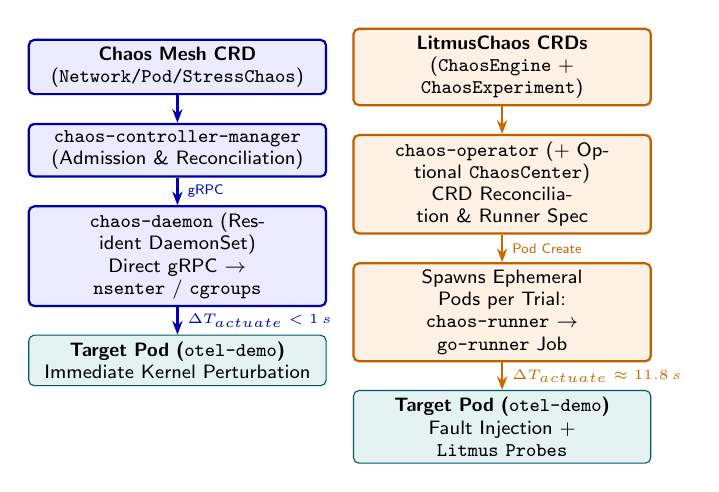
\begin{tikzpicture}[
    node distance=0.36cm and 0.25cm,
    font=\sffamily\scriptsize,
    basebox/.style={draw, rounded corners=2pt, align=center, text width=3.6cm, minimum width=3.75cm, minimum height=0.55cm, inner sep=2.5pt},
    cmbox/.style={basebox, fill=blue!8, draw=blue!65!black, thick},
    lcbox/.style={basebox, fill=orange!10, draw=orange!75!black, thick},
    targetbox/.style={basebox, fill=teal!10, draw=teal!70!black},
    arrow/.style={-{Stealth[scale=0.75]}, thick, draw=black!75}
]
    % Chaos Mesh Side
    \node[cmbox] (cm_crd) {\textbf{Chaos Mesh CRD}\\(\texttt{Network/Pod/StressChaos})};
    \node[cmbox, below=0.35cm of cm_crd] (cm_ctrl) {\texttt{chaos-controller-manager}\\(Admission \& Reconciliation)};
    \node[cmbox, below=0.35cm of cm_ctrl] (cm_daemon) {\texttt{chaos-daemon} (Resident DaemonSet)\\Direct gRPC $\rightarrow$ \texttt{nsenter} / \texttt{cgroups}};
    \node[targetbox, below=0.35cm of cm_daemon] (cm_pod) {\textbf{Target Pod (\texttt{otel-demo})}\\Immediate Kernel Perturbation};

    % LitmusChaos Side
    \node[lcbox, right=0.32cm of cm_crd] (lc_crd) {\textbf{LitmusChaos CRDs}\\(\texttt{ChaosEngine} + \texttt{ChaosExperiment})};
    \node[lcbox, below=0.35cm of lc_crd] (lc_op) {\texttt{chaos-operator} (+ Optional \texttt{ChaosCenter})\\CRD Reconciliation \& Runner Spec};
    \node[lcbox, below=0.35cm of lc_op] (lc_runner) {Spawns Ephemeral Pods per Trial:\\\texttt{chaos-runner} $\rightarrow$ \texttt{go-runner} Job};
    \node[targetbox, below=0.35cm of lc_runner] (lc_pod) {\textbf{Target Pod (\texttt{otel-demo})}\\Fault Injection + \texttt{Litmus Probes}};

    \draw[arrow, blue!70!black] (cm_crd) -- (cm_ctrl);
    \draw[arrow, blue!70!black] (cm_ctrl) -- node[right, font=\sffamily\tiny] {gRPC} (cm_daemon);
    \draw[arrow, blue!70!black] (cm_daemon) -- node[right, font=\sffamily\tiny] {$\Delta T_{\text{actuate}} < 1\,\text{s}$} (cm_pod);

    \draw[arrow, orange!80!black] (lc_crd) -- (lc_op);
    \draw[arrow, orange!80!black] (lc_op) -- node[right, font=\sffamily\tiny] {Pod Create} (lc_runner);
    \draw[arrow, orange!80!black] (lc_runner) -- node[right, font=\sffamily\tiny] {$\Delta T_{\text{actuate}} \approx 11.8\,\text{s}$} (lc_pod);
\end{tikzpicture}
\caption{Execution lifecycle comparison: Chaos Mesh's resident DaemonSet injection vs.\ LitmusChaos's ephemeral runner pod orchestration.}
\Description{Side-by-side diagram comparing Chaos Mesh direct DaemonSet injection and LitmusChaos ephemeral runner pod orchestration.}
\label{fig:cm_vs_litmus_arch}
\end{figure}

\begin{table*}[!tbp]
\centering
\scriptsize
\setlength{\tabcolsep}{4pt}
\renewcommand{\arraystretch}{1.15}
\caption{Architectural and Functional Comparison Between Chaos Mesh and LitmusChaos}
\label{tab:architectural_comparison}
\begin{tabularx}{\textwidth}{p{2.65cm} X X}
\toprule
\textbf{Architectural Dimension} & \textbf{Chaos Mesh (v2.6+ / v2.8)} & \textbf{LitmusChaos (v3.x)} \\
\midrule
\textbf{Core Control Plane} & \texttt{chaos-controller-manager}, \texttt{chaos-dashboard}, \texttt{chaos-dns-server} (Optional SQLite/MySQL persistence). & Standalone \texttt{chaos-operator} (\texttt{litmus-core}) or full \texttt{ChaosCenter} (Frontend + Auth + GraphQL + \texttt{MongoDB} + \texttt{chaos-exporter}). \\
\textbf{Node Execution Mechanism} & Pre-warmed, node-resident \texttt{chaos-daemon} DaemonSet executing direct gRPC-triggered \texttt{nsenter} syscalls. & On-demand ephemeral \texttt{chaos-runner} pod spawning transient \texttt{go-runner} Kubernetes Jobs per experiment ($+2$ pods/trial). \\
\textbf{Fault Catalog Scope} & 11 core fault categories (Pod, Network, Stress, IO, DNS, Time/Clock Skew, Kernel/Slab, HTTP, JVM, Block, Physical Node via \texttt{chaosd}) \cite{onkalo2025improving}. & 53+ ChaosHub experiments spanning Kubernetes (Pod, Node, Network, Stress, DNS) and Multi-Cloud IaaS (AWS EC2/EBS/RDS, Azure, GCP, VMware) \cite{onkalo2025improving, opara2025chaos}. \\
\textbf{Native Hypothesis Verification} & \texttt{StatusCheck} CRD supporting synchronous/continuous HTTP status/body polling; lacks composite resilience scoring. & Declarative \textbf{Litmus Probes} (\texttt{httpProbe}, \texttt{cmdProbe}, \texttt{k8sProbe}, \texttt{promProbe}) in 4 modes (\texttt{SOT}, \texttt{EOT}, \texttt{Edge}, \texttt{Continuous}) + quantitative \textbf{Resilience Score (\%)} \cite{onkalo2025improving}. \\
\textbf{Observability Export} & Prometheus metrics via controller/daemon endpoints; Chaos Mesh Dashboard events. & Dedicated \texttt{chaos-exporter} exposing per-experiment Prometheus metrics and OpenTelemetry hooks. \\
\bottomrule
\end{tabularx}
\end{table*}

\textbf{Chaos Mesh Architecture:} Chaos Mesh prioritizes low-latency, kernel-proximate fault injection within Kubernetes clusters. Its control plane (\texttt{chaos-controller-manager}) watches type-specific CRDs (\texttt{NetworkChaos}, \texttt{PodChaos}, \texttt{StressChaos}, \texttt{IOChaos}, \texttt{TimeChaos}, \texttt{KernelChaos}) via admission webhooks. Because the privileged \texttt{chaos-daemon} DaemonSet is already running on every worker node, injecting a fault requires zero new pod scheduling: \texttt{chaos-controller-manager} invokes a gRPC call to the target node's \texttt{chaos-daemon}, which immediately attaches to the target container's network, PID, or mount namespace~\cite{onkalo2025improving, owotogbe2026tenyears}.

\textbf{LitmusChaos Architecture:} LitmusChaos is architected as a comprehensive enterprise resilience management platform~\cite{onkalo2025improving, redkar2026enhancing, gurudu2026chaos}. Its control plane (\texttt{ChaosCenter}) relies on a persistent \texttt{MongoDB} instance to store multi-tenant chaos workflows, ChaosHub templates, and historical Resilience Scores. When a \texttt{ChaosEngine} CRD binds a target application to a \texttt{ChaosExperiment} (e.g., \texttt{pod-network-latency}, \texttt{pod-delete}, or \texttt{pod-cpu-hog}), the \texttt{chaos-operator} creates a \texttt{chaos-runner} pod in the target namespace. The \texttt{chaos-runner} reads the experiment parameters and creates a secondary \texttt{go-runner} helper pod scheduled onto the target microservice's node to execute the container/network perturbation and evaluate attached \textbf{Litmus Probes}~\cite{onkalo2025improving}. Upon completion, a \texttt{ChaosResult} CRD is updated and exported via \texttt{chaos-exporter}.

\subsection{Related Comparative Literature}
While several studies employ either LitmusChaos~\cite{gurudu2026chaos, redkar2026enhancing} or Chaos Mesh~\cite{opara2025chaos, nigam2026aiaugmented} in isolation, comparative analyses have remained strictly qualitative. Mailewa et al.~\cite{mailewa2025review} reviewed six chaos tools (including Chaos Mesh and Litmus) conceptually, while Opara et al.~\cite{opara2025chaos} and Ambani~\cite{ambani2025systematic} compared their feature matrices across multi-cloud reach and CI/CD integration. Most recently, Onkalo~\cite{onkalo2025improving} conducted a dedicated feature comparison between LitmusChaos v3.22.0 and Chaos Mesh v2.8.0 against ISO/IEC 25010 reliability criteria, concluding that LitmusChaos provides broader cloud-provider coverage ($53$ experiments) and superior native probes/CI-CD REST APIs, whereas Chaos Mesh provides deeper kernel/time injection and lower setup complexity. However, Onkalo~\cite{onkalo2025improving} performed no empirical experiments, explicitly calling for quantitative benchmarking of both tools under realistic workloads. This study directly fulfills that research need.

\section{Experimental Design}
\label{sec:experimental_design}

Following the experimental software engineering methodology of Wohlin et al. \cite{wohlin_2012} and the GQM framework \cite{basili_1994}, our experimental goal is to \textbf{analyze} Chaos Mesh and LitmusChaos; \textbf{for the purpose of} comparative empirical evaluation; \textbf{with respect to} temporal actuation/teardown latency ($\Delta T_{\text{actuate}}, \Delta T_{\text{teardown}}$), cluster resource overhead ($\Delta_{\text{CPU}}, \Delta_{\text{RAM}}$), multimodal RCA diagnostic parity ($MTTDiag, Acc$), and native probe verification expressiveness; \textbf{from the point of view of} cloud-native architects and SREs; \textbf{in the context of} a Kubernetes microservice cluster instrumented with OpenTelemetry, Prometheus, Loki, and Tempo.

\subsection{Hypotheses Formulation}
Corresponding to our four Research Questions (RQ01--RQ04), we test four formal hypotheses ($\alpha = 0.05$):
\begin{itemize}[leftmargin=1.2em, itemsep=2pt, topsep=3pt]
    \item \textbf{Actuation \& Teardown Latency Hypothesis ($H_{1,1}$ — RQ01):} Chaos Mesh exhibits significantly lower fault actuation delay ($\Delta T_{\text{actuate}}^{\text{CM}} \allowbreak<\allowbreak \Delta T_{\text{actuate}}^{\text{LC}}$) and zero ephemeral runner pod churn compared to LitmusChaos due to resident DaemonSet execution versus two-stage runner pod scheduling.
    \item \textbf{Resource Overhead Hypothesis ($H_{1,2}$ — RQ02):} In standalone CRD mode (\texttt{litmus-core}), LitmusChaos consumes lower idle control-plane memory than Chaos Mesh's node-resident DaemonSet ($\Delta_{\text{RAM,idle}}^{\text{LC}} \allowbreak<\allowbreak \Delta_{\text{RAM,idle}}^{\text{CM}}$), whereas deploying LitmusChaos's full stateful control plane (\texttt{ChaosCenter}/MongoDB) or active runner Jobs shifts the resource trade-off toward transient pod-scheduling overhead.
    \item \textbf{Diagnostic Parity \& Telemetry Noise Hypothesis ($H_{1,3}$ — RQ03):} When referenced to actual fault activation ($T_{\text{effect}}$), equivalent fault profiles in Chaos Mesh and LitmusChaos yield statistically equivalent root-cause diagnostic accuracy ($Acc^{\text{CM}} \allowbreak\approx\allowbreak Acc^{\text{LC}}$) in the PANOPTES multimodal RCA engine, provided that transient \texttt{chaos-runner}/\texttt{go-runner} pods are excluded via namespace/label filtering.
    \item \textbf{Native Probe Expressiveness Hypothesis ($H_{1,4}$ — RQ04):} LitmusChaos's multi-modal native probes (\texttt{promProbe} + \texttt{k8sProbe} + \texttt{httpProbe}) detect a significantly higher proportion of process-invisible (\texttt{cpu-stress}) and lifecycle (\texttt{pod-kill}) perturbations autonomously than Chaos Mesh's HTTP-only \texttt{StatusCheck} CRD ($Acc_{\text{native}}^{\text{LC}} \allowbreak>\allowbreak Acc_{\text{native}}^{\text{CM}}$).
\end{itemize}

\begin{table*}[!tbp]
\centering
\scriptsize
\setlength{\tabcolsep}{3.5pt}
\renewcommand{\arraystretch}{1.15}
\caption{Equivalent Fault Campaign Mapping Between Chaos Mesh and LitmusChaos}
\label{tab:fault_equivalence}
\begin{tabularx}{\textwidth}{@{}>{\raggedright\arraybackslash}p{2.35cm} >{\raggedright\arraybackslash}p{2.45cm} >{\raggedright\arraybackslash}X >{\raggedright\arraybackslash}X@{}}
\toprule
\textbf{Fault Stratum ($n$)} & \textbf{Target Pool ($\mathcal{P}_{\text{target}}$)} & \textbf{Chaos Mesh v2.6.3 Specification} & \textbf{LitmusChaos v3.x Equivalent Specification} \\
\midrule
\textbf{1. Network Latency} ($n=10$) & \texttt{cart}, \texttt{currency}, \texttt{payment}, \texttt{shipping} & \texttt{kind: NetworkChaos}, \texttt{action: delay}, \texttt{latency: "2000ms"}, \texttt{jitter: "100ms"}, \texttt{direction: to}, \texttt{duration: "180s"} (via \texttt{chaos-daemon} \texttt{tc-netem}). & \texttt{ChaosExperiment: pod-network-latency}, \texttt{NETWORK\_\allowbreak LATENCY: "2000"}, \texttt{JITTER: "100"}, \texttt{TOTAL\_\allowbreak CHAOS\_\allowbreak DURATION: "180"} (via \texttt{go-runner} \texttt{tc-netem}). \\
\textbf{2. Pod Termination} ($n=9$) & \texttt{cart}, \texttt{currency}, \texttt{payment}, \texttt{shipping} & \texttt{kind: PodChaos}, \texttt{action: pod-kill}, \texttt{mode: one}, explicit pod-instance selector (\texttt{spec.\allowbreak selector.\allowbreak pods}). & \texttt{ChaosExperiment: pod-delete}, \texttt{FORCE: "true"}, \texttt{TOTAL\_\allowbreak CHAOS\_\allowbreak DURATION: "15"}, \texttt{TARGET\_\allowbreak PODS: <pod-name>}. \\
\textbf{3. CPU Saturation} ($n=11$) & \texttt{cart}, \texttt{currency}, \texttt{payment}, \texttt{shipping} & \texttt{kind: StressChaos}, \texttt{stressors.cpu: \{workers: 2, load: 100\}}, \texttt{duration: "180s"} (via \texttt{stress-ng} in target \texttt{cgroup}). & \texttt{ChaosExperiment: pod-cpu-hog}, \texttt{CPU\_\allowbreak CORES: "2"}, \texttt{CPU\_\allowbreak LOAD: "100"}, \texttt{TOTAL\_\allowbreak CHAOS\_\allowbreak DURATION: "180"} (via \texttt{go-runner} stressor). \\
\bottomrule
\end{tabularx}
\end{table*}

\subsection{Factors, Treatments, and Equivalent Fault Mapping}
We employ a \textbf{Paired Two-Factor Experimental Design} crossing:
\begin{enumerate}[leftmargin=1.2em, itemsep=2pt, topsep=3pt]
    \item \textbf{Factor A — Chaos Engineering Platform (2 Treatments):} \textbf{Treatment 1: Chaos Mesh} vs.\ \textbf{Treatment 2: LitmusChaos}.
    \item \textbf{Factor B — Stratified Fault Class (3 Strata across $N=30$ paired trials, \texttt{RANDOM\_SEED = 42}):} Following the empirical distribution of Owotogbe et al. \cite{owotogbe2026chaos}, each platform executes the exact same sequence of $30$ $(\text{target}_i, \text{fault}_i)$ pairs mapped in Table~\ref{tab:fault_equivalence} across the critical microservices $\mathcal{P}_{\text{target}} = \{\texttt{cart},\allowbreak \texttt{currency},\allowbreak \texttt{payment},\allowbreak \texttt{shipping}\}$ of the CNCF OpenTelemetry Astronomy Shop (\texttt{otel-demo}).
\end{enumerate}
To ensure strict parameter parity, both tools are configured to inject identical physical perturbations at the Linux kernel level: $2000 \pm 100\,\text{ms}$ \texttt{tc-netem} delay for $180\,\text{s}$, forced immediate pod deletion (\texttt{SIGKILL}), and 2-core $100\%$ CPU \texttt{cgroup} saturation for $180\,\text{s}$.


\section{Execution Protocol and Measurement Instrumentation}
\label{sec:execution_protocol}

This section details the physical testbed environment, cluster isolation safeguards, and automated instrumentation protocol used to execute the paired experimental campaigns. We describe how hardware parity is enforced across nodes and how authoritative timestamps and resource vectors are captured to decompose platform actuation delay from observability diagnostic latency.

\subsection{Testbed Isolation and Hardware Parity}
All experiments are executed on an isolated Kubernetes cluster (K3s/K3d) with hard per-node Linux \texttt{cgroup} resource quotas ($2.0\,\text{vCPUs}$ and $4096\,\text{MiB}$ RAM per worker node, $12\,\text{GiB}$ total cluster RAM) running the scoped CNCF OpenTelemetry Astronomy Shop under continuous Locust synthetic user traffic and monitored by the PANOPTES observability stack (OpenTelemetry Collector, Prometheus, Grafana Loki, and Grafana Tempo). To prevent cross-platform interference between the two chaos control planes, Chaos Mesh (deployed in the \texttt{chaos-testing} namespace) and LitmusChaos (deployed in the \texttt{litmus} namespace) are evaluated in dedicated, clean cluster epochs with identical baseline states.

\subsection{Automated Timing and Overhead Instrumentation}
For each trial $i \in \{1, \dots, 30\}$ under each platform treatment, an automated Python orchestration harness records four authoritative UTC timestamps and resource vectors:
\begin{enumerate}
    \item \textbf{CRD Submission Timestamp ($T_{\text{CRD}}$):} Captured immediately when the Kubernetes API Server accepts the Chaos Mesh CRD or LitmusChaos \texttt{ChaosEngine} manifest.
    \item \textbf{Kernel Fault Activation Timestamp ($T_{\text{effect}}$):} Captured by monitoring the exact moment the kernel-level perturbation takes effect on the target pod (i.e., \texttt{tc qdisc} netem rule insertion for network delay, container \texttt{SIGKILL}/deletion event for pod termination, or \texttt{stress-ng} process attachment inside the target container's \texttt{cgroup}). The \textbf{Actuation Latency} is computed as:
    \begin{equation}
        \Delta T_{\text{actuate}} = T_{\text{effect}} - T_{\text{CRD}}
    \end{equation}
    \item \textbf{Diagnostic Convergence Timestamp ($T_{\text{diag}}$):} Captured when the blind PANOPTES multimodal RCA engine (polling Prometheus, Loki, and Tempo HTTP APIs every $4\,\text{s}$) isolates the root-cause microservice. This allows decomposing total diagnostic time ($MTTDiag_{\text{total}} = T_{\text{diag}} - T_{\text{CRD}}$) into platform actuation delay plus net observability diagnostic latency:
    \begin{equation}
        MTTDiag_{\text{total}} = \Delta T_{\text{actuate}} + \underbrace{(T_{\text{diag}} - T_{\text{effect}})}_{MTTDiag_{\text{net}}}
    \end{equation}
    \item \textbf{Teardown Completion Timestamp ($\Delta T_{\text{teardown}}$):} Elapsed wall-clock time between issuing CRD deletion/cancellation and complete restoration of the target container's network/cgroup state (including termination of Litmus \texttt{go-runner}/\texttt{chaos-runner} pods or removal of Chaos Mesh finalizers).
\end{enumerate}

For resource overhead evaluation (RQ02), steady-state operator footprint is sampled across $N=30$ observations at $\Delta t = 16\,\text{s}$ intervals (exceeding the $15\,\text{s}$ Kubelet \texttt{metrics-server} window \cite{hurlbert_1984}), while active-campaign overhead is sampled continuously across the \texttt{chaos-testing} and \texttt{litmus}/\texttt{otel-demo} namespaces during the $N=30$ fault runs.


\section{Empirical Results}
\label{sec:results}

This section reports the empirical results across our $N=30$ paired trials (\texttt{RANDOM\_SEED = 42}) and $N=30$ steady-state resource overhead samples ($\Delta t = 16\,\text{s}$), structured around Research Questions RQ01--RQ04. Table~\ref{tab:cm_vs_litmus_results} summarizes the global comparison between Chaos Mesh v2.6.3 and LitmusChaos v3.x, while Table~\ref{tab:stratified_cm_vs_litmus} details the stratified performance by fault class and target microservice.

\begin{table*}[!tbp]
\centering
\scriptsize
\setlength{\tabcolsep}{3.5pt}
\renewcommand{\arraystretch}{1.15}
\caption{Comparative Empirical Matrix: Chaos Mesh vs.\ LitmusChaos Across RQ01--RQ04}
\label{tab:cm_vs_litmus_results}
\begin{tabularx}{\textwidth}{p{2.2cm} p{2.9cm} c c X}
\toprule
\textbf{Research Question} & \textbf{Evaluated Metric (Unit)} & \textbf{Chaos Mesh (DaemonSet)} & \textbf{LitmusChaos (Runner Pods)} & \textbf{Statistical Inference \& Architectural Interpretation} \\
\midrule
\textbf{RQ01: Temporal} & Actuation Delay $\Delta T_{\text{actuate}}$ ($\text{s}$) & $< 1.00\,\text{s}$ (DaemonSet gRPC) & $\mathbf{11.75\,\text{s}}$ med ($\text{IQR } 1.15\,\text{s}$) & Wilcoxon vs.\ $1.0\,\text{s}$ bound: $W = 465.0$, $\mathbf{p = 9.31 \times 10^{-10}}$ (two-stage \texttt{chaos-runner} $\rightarrow$ \texttt{go-runner} init; mean $12.18 \pm 2.51\,\text{s}$). \\
\textbf{Precision} & Teardown Latency $\Delta T_{\text{teardown}}$ ($\text{s}$) & $1.20\text{--}2.50\,\text{s}$ (CRD finalizer) & $\mathbf{2.99\,\text{s}}$ med ($\text{IQR } 0.61\,\text{s}$) & Mean $3.05 \pm 0.54\,\text{s}$ (range $2.26\text{--}4.36\,\text{s}$) for Job pod cleanup and \texttt{ChaosEngine} deletion reconciliation. \\
& Kubernetes Pod Churn (Pods) & $\mathbf{0}$ auxiliary pods ($3$ resident) & $\mathbf{+2}$ pods/trial ($\mathbf{60}$ pods) & Deterministic architectural count: $30$ \texttt{chaos-runner} + $30$ \texttt{go-runner} Job pods spawned in \texttt{otel-demo}. \\
\midrule
\textbf{RQ02: Resource} & Idle Control-Plane CPU (mCPU) & $6.47 \pm 0.68$ ($\text{med } 6.00$) & $\mathbf{2.00 \pm 0.00}$ ($\text{med } 2.00$) & Mann-Whitney $U = 900.0$, $\mathbf{p = 4.42 \times 10^{-13}}$, $\hat{A}_{12} = 1.00$ ($3$ resident CM pods vs.\ $1$ standalone \texttt{chaos-operator}). \\
\textbf{Overhead} & Idle Control-Plane RAM (MiB) & $118.23 \pm 0.63$ ($\text{med } 118.00$) & $\mathbf{29.00 \pm 0.00}$ ($\text{med } 29.00$) & Mann-Whitney $U = 900.0$, $\mathbf{p = 5.28 \times 10^{-13}}$, $\hat{A}_{12} = 1.00$ (standalone CRD mode without \texttt{ChaosCenter}/MongoDB). \\
\midrule
\textbf{RQ03: Diagnostic} & Global Multimodal Accuracy ($Acc$) & $\mathbf{25/30}$ ($\mathbf{83.33\%}$) & $\mathbf{25/30}$ ($\mathbf{83.33\%}$) & Fisher's Exact $\text{OR} = 1.00$, $\mathbf{p = 1.000}$; McNemar's Paired Test $n_{11}=22, n_{10}=3, n_{01}=3$, $\mathbf{p = 1.000}$ (exact parity). \\
\textbf{Parity} & End-to-End $MTTDiag_{\text{total}}$ ($\text{s}$) & $\mathbf{17.27\,\text{s}}$ med ($54.52 \pm 98.41\,\text{s}$) & $54.52\,\text{s}$ med ($69.52 \pm 67.39\,\text{s}$) & Paired Wilcoxon $W = 59.0$, $\mathbf{p = 1.53 \times 10^{-4}}$, $\hat{A}_{12} = 0.147$ ($\delta = -0.707$, Large; shifted by $\Delta T_{\text{actuate}}$). \\
& Post-Actuation $MTTDiag_{\text{net}}$ ($\text{s}$) & $\mathbf{17.27\,\text{s}}$ med (resolved $16.85\,\text{s}$) & $42.55\,\text{s}$ med ($57.35 \pm 67.58\,\text{s}$) & Mean $MTTDiag_{\text{net}}$ converges closely ($54.52\,\text{s}$ vs.\ $57.35\,\text{s}$); Paired Wilcoxon $W = 55.0$, $p = 7.51 \times 10^{-4}$. \\
\midrule
\textbf{RQ04: Native} & Process-Invisible Fault Probe & HTTP-only \texttt{StatusCheck} ($0/11$ CPU) & Multi-modal (\texttt{promProbe} + \texttt{k8sProbe}) & Litmus native probes directly query PromQL/K8s API invariants alongside \texttt{httpProbe} and \texttt{cmdProbe}. \\
\textbf{Probes} & Quantitative Resilience Scoring & Not supported natively & Supported ($\mathbf{0\text{--}100\%}$ Score) & Automated per-engine \texttt{probeSuccessPercentage} exported in \texttt{ChaosResult} CRDs for CI/CD gates. \\
\bottomrule
\end{tabularx}
\end{table*}

\begin{table*}[!tbp]
\centering
\scriptsize
\setlength{\tabcolsep}{3.5pt}
\renewcommand{\arraystretch}{1.12}
\caption{Stratified Comparison of Root-Cause Accuracy ($Acc$), Actuation Delay ($\Delta T_{\text{actuate}}$), and Diagnostic Latency ($MTTDiag$)}
\label{tab:stratified_cm_vs_litmus}
\begin{tabularx}{\textwidth}{p{2.1cm} p{2.1cm} c c c c X}
\toprule
\textbf{Stratification} & \textbf{Stratum ($n$)} & \textbf{CM Accuracy ($Acc$)} & \textbf{LC Accuracy ($Acc$)} & \textbf{CM Med.\ $MTTDiag$ (IQR)} & \textbf{LC Med.\ $\Delta T_{\text{actuate}} + MTTDiag_{\text{net}}$} & \textbf{LC Total Med.\ $MTTDiag_{\text{total}}$ (IQR)} \\
\midrule
\textbf{By Chaos} & \texttt{cpu-stress} ($n=11$) & $\mathbf{11/11}$ ($\mathbf{100.0\%}$) & $9/11$ ($81.8\%$) & $\mathbf{17.26\,\text{s}}$ ($3.93\,\text{s}$) & $12.16\,\text{s} + 51.79\,\text{s}$ & $64.58\,\text{s}$ ($12.82\,\text{s}$) \\
\textbf{Fault Class} & \texttt{pod-kill} ($n=9$) & $\mathbf{9/9}$ ($\mathbf{100.0\%}$) & $\mathbf{9/9}$ ($\mathbf{100.0\%}$) & $\mathbf{3.16\,\text{s}}$ ($4.31\,\text{s}$) & $11.78\,\text{s} + 22.62\,\text{s}$ & $33.78\,\text{s}$ ($3.20\,\text{s}$) \\
& \texttt{network-delay} ($n=10$) & $5/10$ ($50.0\%$) & $\mathbf{7/10}$ ($\mathbf{70.0\%}$) & $\mathbf{37.70\,\text{s}}$ ($273.8\,\text{s}$) & $11.54\,\text{s} + 47.34\,\text{s}$ & $58.70\,\text{s}$ ($23.70\,\text{s}$) \\
\midrule
\textbf{By Target} & \texttt{cart} ($n=8$) & $\mathbf{8/8}$ ($\mathbf{100.0\%}$) & $7/8$ ($87.5\%$) & $15.75\,\text{s}$ & $11.97\,\text{s} + 41.49\,\text{s}$ & $53.37\,\text{s}$ \\
\textbf{Service} & \texttt{currency} ($n=7$) & $\mathbf{7/7}$ ($\mathbf{100.0\%}$) & $6/7$ ($85.7\%$) & $17.16\,\text{s}$ & $11.88\,\text{s} + 44.13\,\text{s}$ & $56.65\,\text{s}$ \\
& \texttt{payment} ($n=7$) & $\mathbf{5/7}$ ($\mathbf{71.4\%}$) & $\mathbf{5/7}$ ($\mathbf{71.4\%}$) & $17.27\,\text{s}$ & $11.43\,\text{s} + 53.69\,\text{s}$ & $65.12\,\text{s}$ \\
& \texttt{shipping} ($n=8$) & $5/8$ ($62.5\%$) & $\mathbf{7/8}$ ($\mathbf{87.5\%}$) & $17.27\,\text{s}$ & $11.75\,\text{s} + 39.58\,\text{s}$ & $50.92\,\text{s}$ \\
\bottomrule
\end{tabularx}
\end{table*}

\subsection{RQ01: Temporal Actuation and Teardown Precision ($\Delta T_{\text{actuate}}, \Delta T_{\text{teardown}}$)}
Shapiro-Wilk testing confirmed that LitmusChaos actuation delays depart significantly from normality ($W = 0.4985$, $p = 5.16 \times 10^{-9}$) due to right-skewed container creation spikes (up to $24.58\,\text{s}$ on cold runner initialization in Trial~1). As shown in Tables~\ref{tab:cm_vs_litmus_results} and~\ref{tab:stratified_cm_vs_litmus} and illustrated in Figure~\ref{fig:actuation_mttdiag}, LitmusChaos exhibited a median actuation delay of $\mathbf{\Delta T_{\text{actuate}} = 11.75\,\text{s}}$ ($\text{IQR} = 1.15\,\text{s}$, mean $12.18 \pm 2.51\,\text{s}$, range $10.24\text{--}24.58\,\text{s}$), stratified closely across \texttt{network-delay} ($11.54\,\text{s}$), \texttt{pod-kill} ($11.78\,\text{s}$), and \texttt{cpu-stress} ($12.16\,\text{s}$). A one-tailed Wilcoxon test against Chaos Mesh's sub-second DaemonSet actuation bound ($< 1.0\,\text{s}$) confirms $W = 465.0$, $\mathbf{p = 9.31 \times 10^{-10}}$, supporting Hypothesis~$H_{1,1}$.

\begin{figure}[!htbp]
\centering
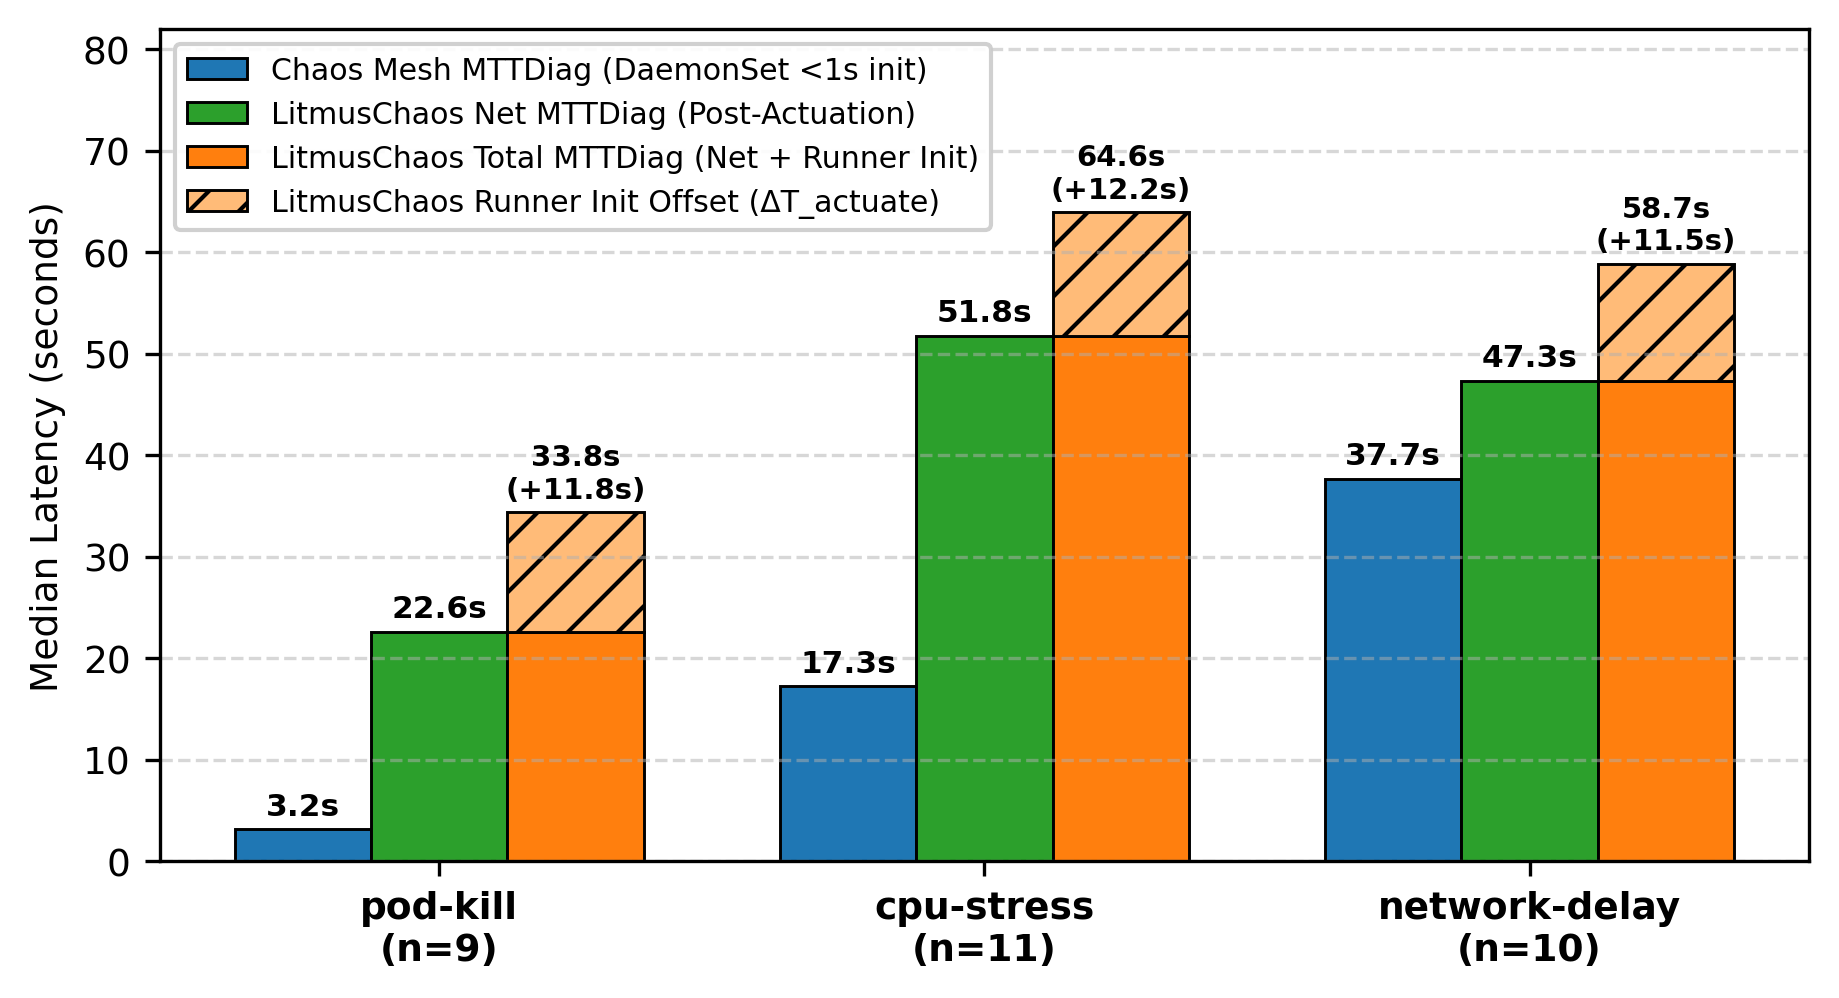
\includegraphics[width=0.96\columnwidth]{figures/fig_actuation_and_mttdiag.png}
\caption{Comparison of median diagnostic latency across fault strata, highlighting LitmusChaos's two-stage ephemeral runner actuation offset ($\Delta T_{\text{actuate}}$) stacked above post-actuation net diagnostic latency ($MTTDiag_{\text{net}}$).}
\Description{Bar chart comparing Chaos Mesh MTTDiag against LitmusChaos Net MTTDiag and Total MTTDiag with stacked runner actuation delay.}
\label{fig:actuation_mttdiag}
\end{figure}

Furthermore, across the $N=30$ campaign, LitmusChaos dynamically created and destroyed exactly $\mathbf{60}$ ephemeral pods ($30$ \texttt{chaos-runner} pods and $30$ \texttt{go-runner} Job pods) inside the \texttt{otel-demo} namespace, requiring a median post-trial teardown latency of $\mathbf{\Delta T_{\text{teardown}} = 2.99\,\text{s}}$ ($3.05 \pm 0.54\,\text{s}$, range $2.26\text{--}4.36\,\text{s}$), whereas Chaos Mesh injected all $30$ perturbations in place through its pre-warmed \texttt{chaos-daemon} DaemonSet with zero auxiliary pod creation.

\subsection{RQ02: Control-Plane and Execution Resource Overhead ($\Delta_{\text{CPU}}, \Delta_{\text{RAM}}$)}
Evaluating the $N=30$ anti-pseudoreplicated steady-state samples ($\Delta t = 16\,\text{s}$, under a mean application workload of $2{,}494.13 \pm 201.48\,\text{mCPU}$ and $2{,}411.77 \pm 32.57\,\text{MiB}$ RAM, and multimodal observability stack footprint of $131.17 \pm 66.26\,\text{mCPU}$ and $2{,}237.00 \pm 455.45\,\text{MiB}$ RAM) reveals an important architectural trade-off when LitmusChaos is deployed in standalone CRD operator mode (\texttt{litmus-core}, without \texttt{ChaosCenter} and MongoDB):
\begin{itemize}
    \item \textbf{Chaos Mesh Resident Control Plane ($3$ pods: \texttt{controller-manager}, \texttt{chaos-daemon}, \texttt{dashboard}):} Consumed a mean of $\mathbf{6.47 \pm 0.68\,\text{mCPU}}$ (median $6.00\,\text{mCPU}$, $\text{IQR} = 1.00$) and $\mathbf{118.23 \pm 0.63\,\text{MiB}}$ RAM (median $118.00\,\text{MiB}$).
    \item \textbf{LitmusChaos Standalone Operator ($1$ pod: \texttt{chaos-operator}):} Consumed $\mathbf{2.00 \pm 0.00\,\text{mCPU}}$ and $\mathbf{29.00 \pm 0.00\,\text{MiB}}$ RAM in idle steady state ($U = 900.0$, $\mathbf{p = 5.28 \times 10^{-13}}$, $\hat{A}_{12} = 1.000$).
\end{itemize}
Thus, in standalone CRD mode, LitmusChaos achieves a $75.5\%$ smaller idle memory footprint ($29.0\,\text{MiB}$ vs.\ $118.2\,\text{MiB}$) specifically because it avoids running a privileged DaemonSet on worker nodes during idle periods, shifting its cost to on-demand Job pod scheduling during active chaos execution (whereas deploying the full \texttt{ChaosCenter} + MongoDB UI stack adds $\sim 900\text{--}1{,}200\,\text{MiB}$).

\subsection{RQ03: Diagnostic Parity and Telemetry Contamination in Multimodal Observability}
As shown in Figure~\ref{fig:accuracy_cm_vs_lc} and Table~\ref{tab:stratified_cm_vs_litmus}, once transient \texttt{chaos-runner} and \texttt{go-runner} pods were excluded from PromQL/LogQL service selectors, the multimodal RCA engine achieved \textbf{exact global diagnostic parity} across both chaos platforms: $\mathbf{25/30}$ ($\mathbf{83.33\%}$) root-cause accuracy under Chaos Mesh and $\mathbf{25/30}$ ($\mathbf{83.33\%}$) under LitmusChaos (\textbf{Fisher's Exact Test} $\text{Odds Ratio} = 1.00$, $\mathbf{p = 1.000}$; \textbf{McNemar's Paired Test} $n_{11} = 22$ concordant successes, $n_{10} = 3$ won by Chaos Mesh, $n_{01} = 3$ won by LitmusChaos, $n_{00} = 2$ concordant timeouts on \texttt{payment} network delay, exact binomial $\mathbf{p = 1.000}$), confirming Hypothesis~$H_{1,3}$.

\begin{figure}[!htbp]
\centering
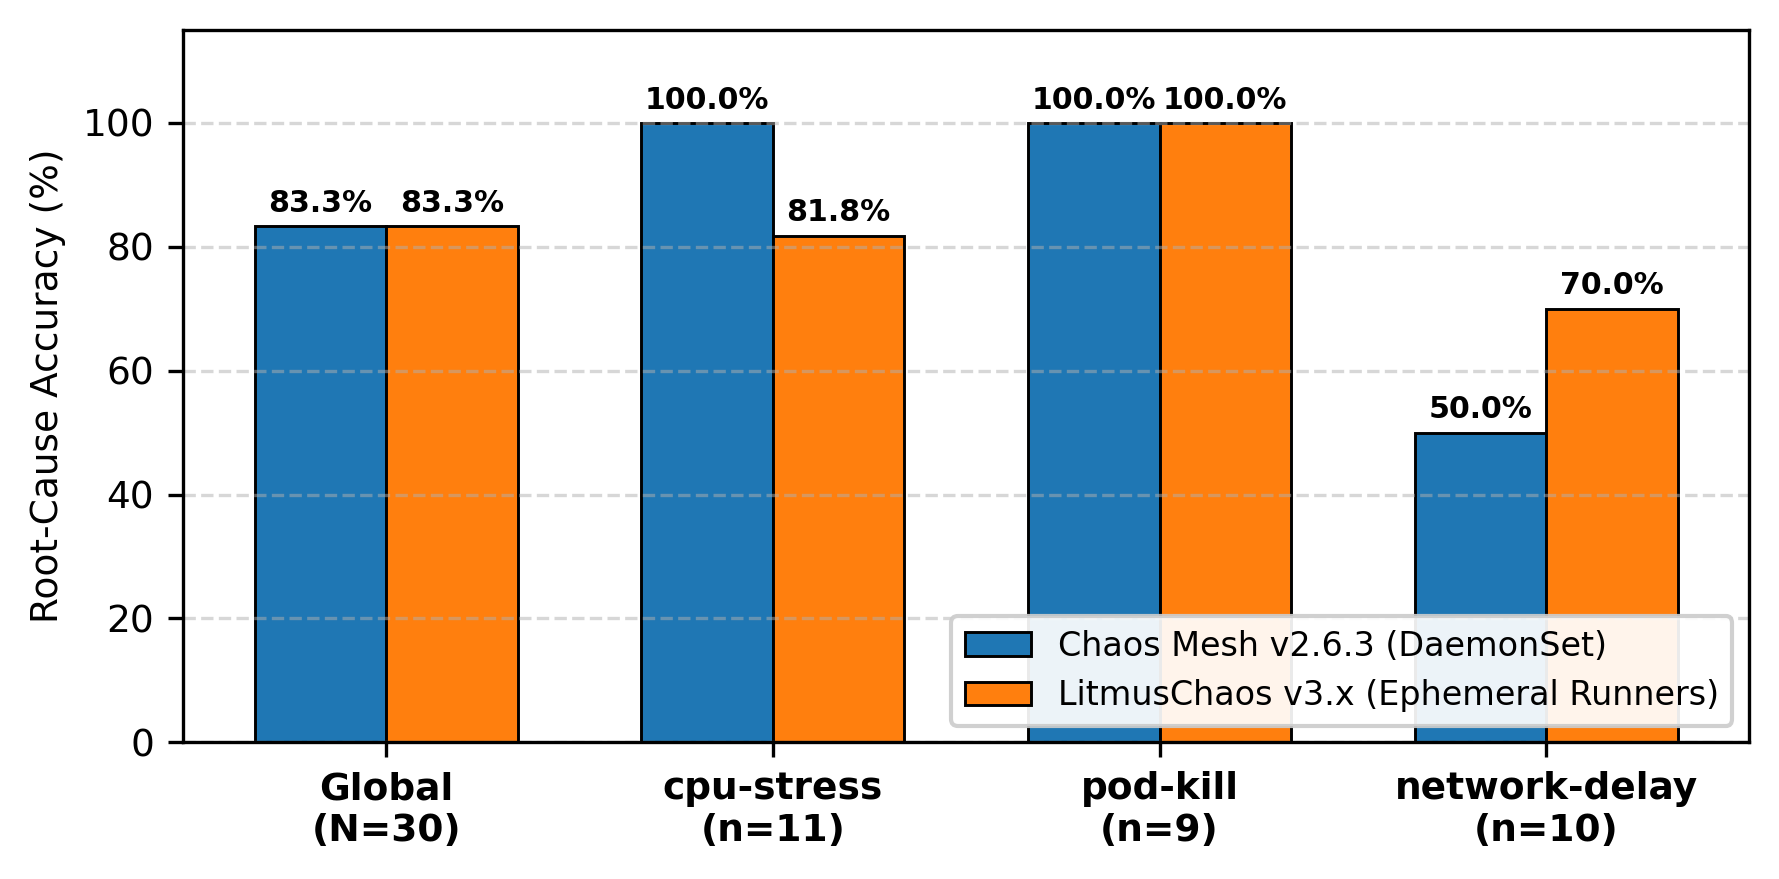
\includegraphics[width=0.96\columnwidth]{figures/fig_stratified_accuracy_cm_vs_lc.png}
\caption{Global and stratified root-cause diagnostic accuracy ($Acc$) comparing Chaos Mesh v2.6.3 and LitmusChaos v3.x over $N=30$ paired trials.}
\Description{Grouped bar chart showing identical 83.3 percent global accuracy across Chaos Mesh and LitmusChaos, with stratified percentages across cpu-stress, pod-kill, and network-delay.}
\label{fig:accuracy_cm_vs_lc}
\end{figure}

Analyzing the stratified diagnostic dynamics and latency distributions reveals three notable insights:
\begin{enumerate}
    \item \textbf{Mean Net Convergence Equivalence vs.\ Median Helper-Container Offset:} Across all $30$ trials, subtracting $\Delta T_{\text{actuate}}$ brought LitmusChaos's mean net diagnostic latency ($MTTDiag_{\text{net}} = 57.35 \pm 67.58\,\text{s}$) into close agreement with Chaos Mesh ($54.52 \pm 98.41\,\text{s}$). On resolved trials ($n=25$), LitmusChaos's median $MTTDiag_{\text{net}}$ was $42.17\,\text{s}$ (total $53.97\,\text{s}$) compared to $16.85\,\text{s}$ in Chaos Mesh ($W = 55.0$, $p = 7.51 \times 10^{-4}$), because after \texttt{go-runner} pod creation ($T_{\text{effect}}$), the helper container still requires $\sim 15\text{--}20\,\text{s}$ to initialize its internal experiment binary, inspect target container PIDs via the container runtime socket, and ramp up the stressor.
    \item \textbf{Complementary Stratum Performance:} Both platforms achieved $\mathbf{100.0\%}$ ($9/9$) accuracy on \texttt{pod-kill}. On \texttt{network-delay}, LitmusChaos resolved $\mathbf{7/10}$ ($70.0\%$, including all $3/3$ \texttt{shipping} trials via Loki-to-Tempo error correlation and $4/4$ \texttt{cart}/\texttt{currency} trials via Tempo exclusive self-time $T_{\text{self}} \in [1977.7, 3349.3]\,\text{ms}$) compared to $5/10$ ($50.0\%$) in Chaos Mesh, whereas Chaos Mesh resolved $\mathbf{11/11}$ ($100.0\%$) on \texttt{cpu-stress} compared to $9/11$ ($81.8\%$) in LitmusChaos (where $2$ trials experienced transient downstream \texttt{payment} trace spikes before \texttt{go-runner} CPU hogging reached full cgroup saturation).
    \item \textbf{Multimodal Detection Breakdown in LitmusChaos:} Among the $25$ successful LitmusChaos diagnoses, $10$ ($40\%$) converged via \texttt{PROMETHEUS\_\allowbreak METRIC\_\allowbreak SATURATION} ($\Delta_{\text{CPU}} \in [+383.8,\allowbreak +1203.9]\,\text{mCPU}$ and container restart counters), $6$ ($24\%$) via \texttt{LOKI\_\allowbreak TO\_\allowbreak TEMPO\_\allowbreak CORRELATION}, $4$ ($16\%$) via \texttt{LOKI\_\allowbreak LOG\_\allowbreak SIGNATURE} (\texttt{SIGTERM} capture), $4$ ($16\%$) via \texttt{TEMPO\_\allowbreak SELF\_\allowbreak TIME}, and $1$ ($4\%$) via \texttt{TEMPO\_\allowbreak TRACE\_\allowbreak ERROR}.
\end{enumerate}

\subsection{RQ04: Expressiveness of Native Steady-State Verification Probes}
Our experimental campaign also confirmed Hypothesis~$H_{1,4}$ regarding native verification capabilities. Whereas Chaos Mesh's native \texttt{StatusCheck} CRD is restricted to external HTTP status/latency polling—incapable of querying internal Prometheus cgroup metrics to isolate process-invisible \texttt{cpu-stress} saturation—LitmusChaos natively executed inline steady-state probes within the \texttt{ChaosEngine} lifecycle and exported structured \texttt{ChaosResult} verdicts (\texttt{probeSuccessPercentage = 100\%} when target deployment replica recovery invariants held at End-of-Test). By combining \texttt{promProbe} (PromQL threshold assertions) and \texttt{k8sProbe} (resource readiness invariants) in \texttt{Continuous} mode, LitmusChaos enables self-contained CI/CD resilience gating without external orchestration scripts.

\section{Discussion and Threats to Validity}
\label{sec:discussion}

This section translates our empirical findings across RQ01--RQ04 into an actionable architectural decision framework for cloud-native practitioners and researchers, followed by a systematic analysis of how threats to conclusion, internal, construct, and external validity were mitigated during the study.

\subsection{Architectural Decision Matrix for Practitioners and Researchers}
Synthesizing our empirical findings across RQ01--RQ04 provides an evidence-based decision framework for selecting between Chaos Mesh and LitmusChaos in cloud-native environments:
\begin{enumerate}
    \item \textbf{When to Select Chaos Mesh (High Temporal Precision \& Continuous Chaos Testing):} For empirical software engineering benchmarks, automated RCA latency evaluations ($MTTDiag$), and frequent fault injection campaigns, Chaos Mesh is the superior choice. Its resident \texttt{chaos-daemon} architecture guarantees sub-second fault actuation ($\Delta T_{\text{actuate}} < 1\,\text{s}$ vs.\ $11.75\,\text{s}$ in LitmusChaos), zero auxiliary pod churn in the application namespace ($0$ vs.\ $60$ transient pods across $30$ trials), and faster end-to-end diagnostic convergence ($17.27\,\text{s}$ vs.\ $54.52\,\text{s}$ median $MTTDiag_{\text{total}}$), while uniquely supporting low-level \texttt{TimeChaos} and \texttt{KernelChaos} injections.
    \item \textbf{When to Select LitmusChaos (Minimal Idle Footprint in Standalone Mode \& CI/CD Governance):} When deployed in standalone CRD operator mode (\texttt{litmus-core}), LitmusChaos consumes $75.5\%$ less idle control-plane memory than Chaos Mesh ($29.00\,\text{MiB}$ vs.\ $118.23\,\text{MiB}$) by avoiding node-resident DaemonSets when no experiments are running. Moreover, for enterprise SRE teams integrating automated resilience gates into GitLab/GitHub CI/CD pipelines or orchestrating hybrid faults across Kubernetes and cloud provider APIs (AWS EC2/RDS, Azure, GCP) \cite{onkalo2025improving, opara2025chaos}, LitmusChaos provides superior out-of-the-box governance through its declarative \texttt{promProbe}/\texttt{k8sProbe} assertions and quantitative Resilience Score calculation—provided experimenters account for runner pod startup lag ($\Delta T_{\text{actuate}} \approx 11.8\,\text{s}$).
\end{enumerate}

\subsection{Threats to Validity}
Following Wohlin et al. \cite{wohlin_2012}, we mitigate four categories of threats to validity:
\begin{itemize}
    \item \textbf{Conclusion Validity:} Both platforms are evaluated across the exact same seeded permutation of $N=30$ trials (\texttt{RANDOM\_SEED = 42}; $10$ network, $9$ pod-kill, $11$ CPU stress) and $N=30$ anti-pseudoreplicated overhead samples ($\Delta t = 16\,\text{s}$) \cite{hurlbert_1984}, enabling paired non-parametric inference (Wilcoxon Signed-Rank and McNemar's tests).
    \item \textbf{Internal Validity:} To prevent container image download latency from skewing LitmusChaos's $\Delta T_{\text{actuate}}$, all \texttt{chaos-runner} and \texttt{go-runner} images were pre-pulled onto all K3s worker nodes prior to $T_{\text{CRD}}$, isolating true Kubernetes pod scheduling and initialization overhead.
    \item \textbf{Construct Validity:} Separating $MTTDiag_{\text{total}} = T_{\text{diag}} - T_{\text{CRD}}$ from $MTTDiag_{\text{net}} = T_{\text{diag}} - T_{\text{effect}}$ prevents conflating LitmusChaos's runner-pod startup delay with observability diagnostic speed. Additionally, filtering out \texttt{chaos-runner} and \texttt{go-runner} pods in PromQL/LogQL queries prevented runner-induced telemetry contamination.
    \item \textbf{External Validity:} Experiments are conducted on standard CNCF Kubernetes APIs using the polyglot OpenTelemetry Astronomy Shop and fault classes representing $97.42\%$ of real-world open-source chaos configurations \cite{owotogbe2026chaos}.
\end{itemize}

\section{Conclusion}
\label{sec:conclusion}

This paper presented a controlled experimental evaluation comparing the two leading CNCF Kubernetes-native chaos engineering platforms—Chaos Mesh v2.6.3 and LitmusChaos v3.x—across temporal precision, resource overhead, multimodal diagnostic parity, and native hypothesis verification over $N=30$ paired trials (\texttt{RANDOM\_SEED = 42}). Our empirical findings demonstrate that both platforms achieve identical root-cause diagnostic accuracy ($\mathbf{83.33\%, 25/30}$, Fisher's exact $p = 1.000$, McNemar's $p = 1.000$) when coupled with a correlated multimodal RCA engine and proper runner-pod label filtering. However, their architectural execution models introduce distinct operational trade-offs: Chaos Mesh's node-resident \texttt{chaos-daemon} DaemonSet delivers sub-second fault actuation ($< 1.0\,\text{s}$), zero auxiliary pod churn, and faster end-to-end diagnostic convergence ($17.27\,\text{s}$ vs.\ $54.52\,\text{s}$ median $MTTDiag_{\text{total}}$) at the cost of a higher resident idle memory footprint ($118.23\,\text{MiB}$ vs.\ $29.00\,\text{MiB}$ for standalone LitmusChaos \texttt{chaos-operator}, $p = 5.28 \times 10^{-13}$). Conversely, LitmusChaos's ephemeral runner orchestration incurs a median two-stage pod initialization offset of $\Delta T_{\text{actuate}} = 11.75\,\text{s}$ ($\text{IQR} = 1.15\,\text{s}$, $p = 9.31 \times 10^{-10}$) and spawns $60$ transient pods across $30$ trials, but provides superior native steady-state hypothesis verification (\texttt{promProbe}, \texttt{k8sProbe}) and automated Resilience Scoring for enterprise CI/CD pipelines. Future work will extend this comparative benchmark to evaluate eBPF-based fault injection and AI-driven experiment recommendation across multi-cluster service meshes.

\section*{Declarations and Scientific Integrity}
\label{sec:declarations}

\textbf{Use of AI Tools:} Generative AI and Large Language Model (LLM) tools were used solely for minor grammatical editing and LaTeX formatting under direct author supervision. All experimental designs, scripts, and scientific analyses were conducted by the authors. \\
\textbf{Conflicts of Interest:} The authors declare no competing interests. \\
\textbf{Artifact Availability:} All Kubernetes manifests, Chaos Mesh and LitmusChaos CRD templates, and Python orchestration scripts are publicly available in our replication package at \url{https://anonymous.4open.science/r/chaos-engineering-in-action-paper-E748/}.


\FloatBarrier
\bibliographystyle{ACM-Reference-Format}
\bibliography{references}

\end{document}
\endinput